\chapter{Ideas Sueltas}

\begin{itemize}
    \item Lineas de trabajo
    \begin{itemize}
        \item Crear una extension en jupyter para pyexams
        \item \textbf{Ampliar pyexams para escanear exámenes impresos}
        \begin{itemize}
            \item \textbf{Obtener las casillas y solución}
            \item Escanear exámenes y obtener la información de las casillas
            \item Identificación de casillas marcadas
            \item Puntuar
        \end{itemize}
    \end{itemize}
    \item Issues de framagit
    \begin{itemize}
        \item Issue 1: Choosing all variants from a list instead of random numbers
        \item \textbf{Issue 2: pyexams --prepare-send, pyexams --prepare-exam}
        \item Issue 3: export to jupyter notebook
        \item Issue 4: sort questions in alphabetical order
        \item Issue 5: `pyexams -send` receives also extra argument students.csv
        \item Issue 6: print the output of pdflatex properly if there is an error
    \end{itemize}
    \item Documentación del TFG
    \begin{itemize}
        \item Definir distintos tipos de preguntas que acepta pyexams
        \item Diagrama de componentes/clases
        \item \textbf{Lista de requisitos} -> Hacer una entrevista de requisitos en navales
        \item Metodologías Ágiles -> sacar de la Bitácora y la lista de requisitos los sprints
        \item Definir los conocimientos utilizados para la realización del TFG y de donde se ha obtenido 
        \item \textbf{Documentar las pruebas realizadas con imágenes}
        \item Utilización de cuadernos jupyter para la realización de pruebas
    \end{itemize}
\end{itemize}

Componentes de la función Escanear Exámenes:

\begin{figure}
    \centering
    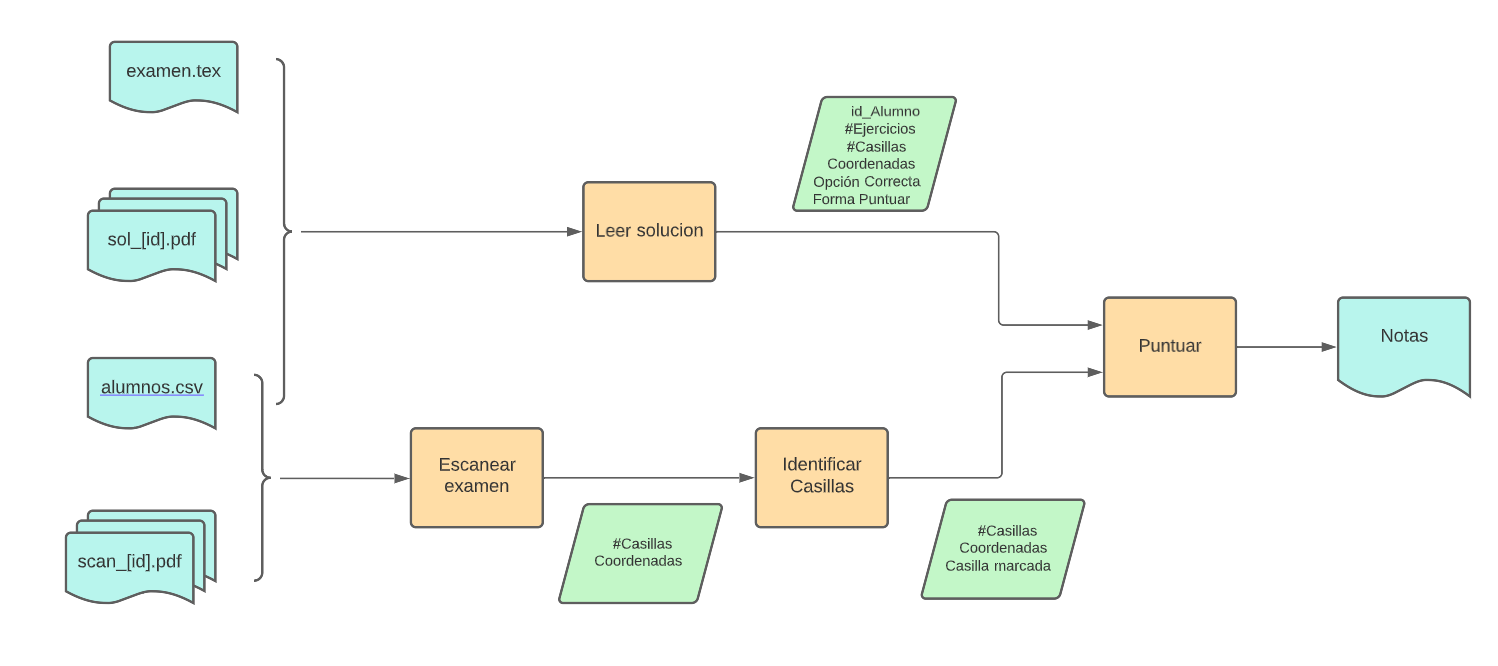
\includegraphics[width=0.9\textwidth]{figures/componentes_escanear1.png}
    \caption{Diagrama de componentes inicial}
    \label{fig:diagrama1}
\end{figure}

(Diagrama de componentes inicial, con la herramienta lucid.app en \href{https://lucid.app/lucidchart/e4e3ac39-6d50-46bd-bb09-bdcd95795a17/edit?beaconFlowId=4856D1B22948543C&invitationId=inv_6249bed2-3464-41f5-808e-d6051f99857c&page=0_0#}{este enlace}.)

\begin{itemize}
    \item  Escanear examenes
\end{itemize}
\textit{La funcionalidad Escanear exámenes obtiene las siguientes entradas: unos exámenes escaneados en formato [\_], el fichero alumnos.csv, los pdf con la solución generada por pyexams y [\_]. A partir de estas entradas debe, para cada alumno de alumnos.csv, obtener los datos de la solución, procesar los exámenes escaneados para identificar las casillas, si están marcadas, puntuar los exámenes y generar un archivo con las notas de todos estos.}

\begin{itemize}
    \item Leer solución: Obtiene de la solución la posición de las casillas y si están marcadas.
    \item Escanear examen: Obtiene de los exámenes escaneados las casillas
    \item Identificar casillas: Analiza si las casillas leídas por escanear exámenes están marcadas
    \item Puntuar: A partir del estado de las casillas de la solución y del examen escaneado puntúa el examen ¿forma de puntuar?
\end{itemize}

Pruebas de Escanear Examenes

\begin{itemize}
    \item Creado un banco de pruebas con el ejemplo de python3/en, añadiendo alumnos
    \begin{itemize}
        \item Generado los statements y solutions con pyexams
\begin{figure}
    \centering
    \begin{minipage}{.5\textwidth}
        \centering
        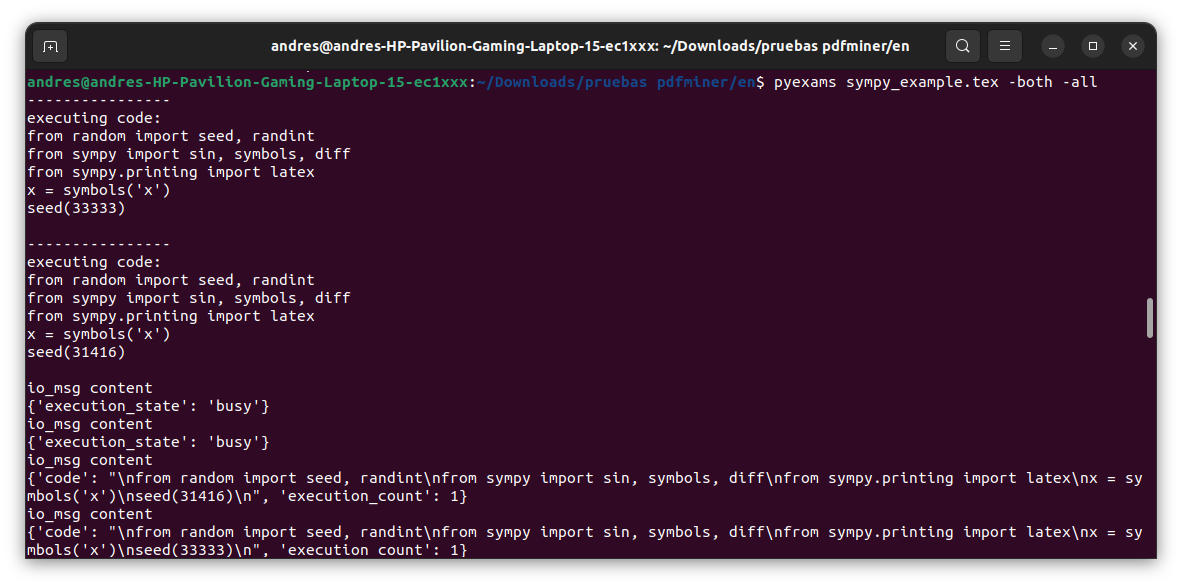
\includegraphics[width=0.9\textwidth]{figures/exec_py_banco.png}
        \caption{Ejecución de pyexams}
        \label{fig:run_banc}
    \end{minipage}%
    \begin{minipage}{.5\textwidth}
        \centering
        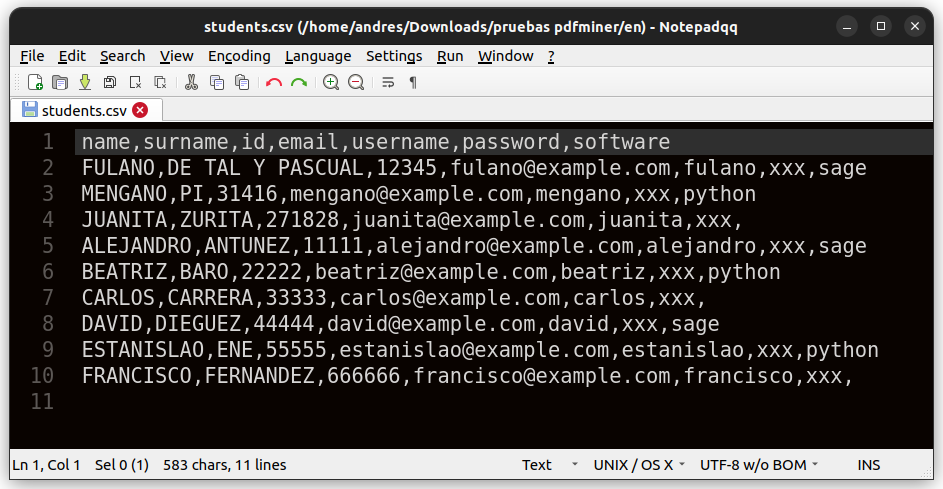
\includegraphics[width=0.9\textwidth]{figures/alum_banco.png}
        \caption{Lista de alumnos}
        \label{fig:aluml_banc}
    \end{minipage}
\end{figure}
        \item Rellenado los statements con un editor de pdf
        \item Generado escaneados de los statements con \href{https://www.i2pdf.com/pdf-to-scan/}{i2pdf}. Esta herramienta permite ajustar la cantidad de ruido, la cantidad de giro y los dpi (dots per inch).
        \begin{itemize}
            \item Los pdfs generados no dibujan las casillas (\ref{fig:fscan_bad})
\begin{figure}
    \centering
    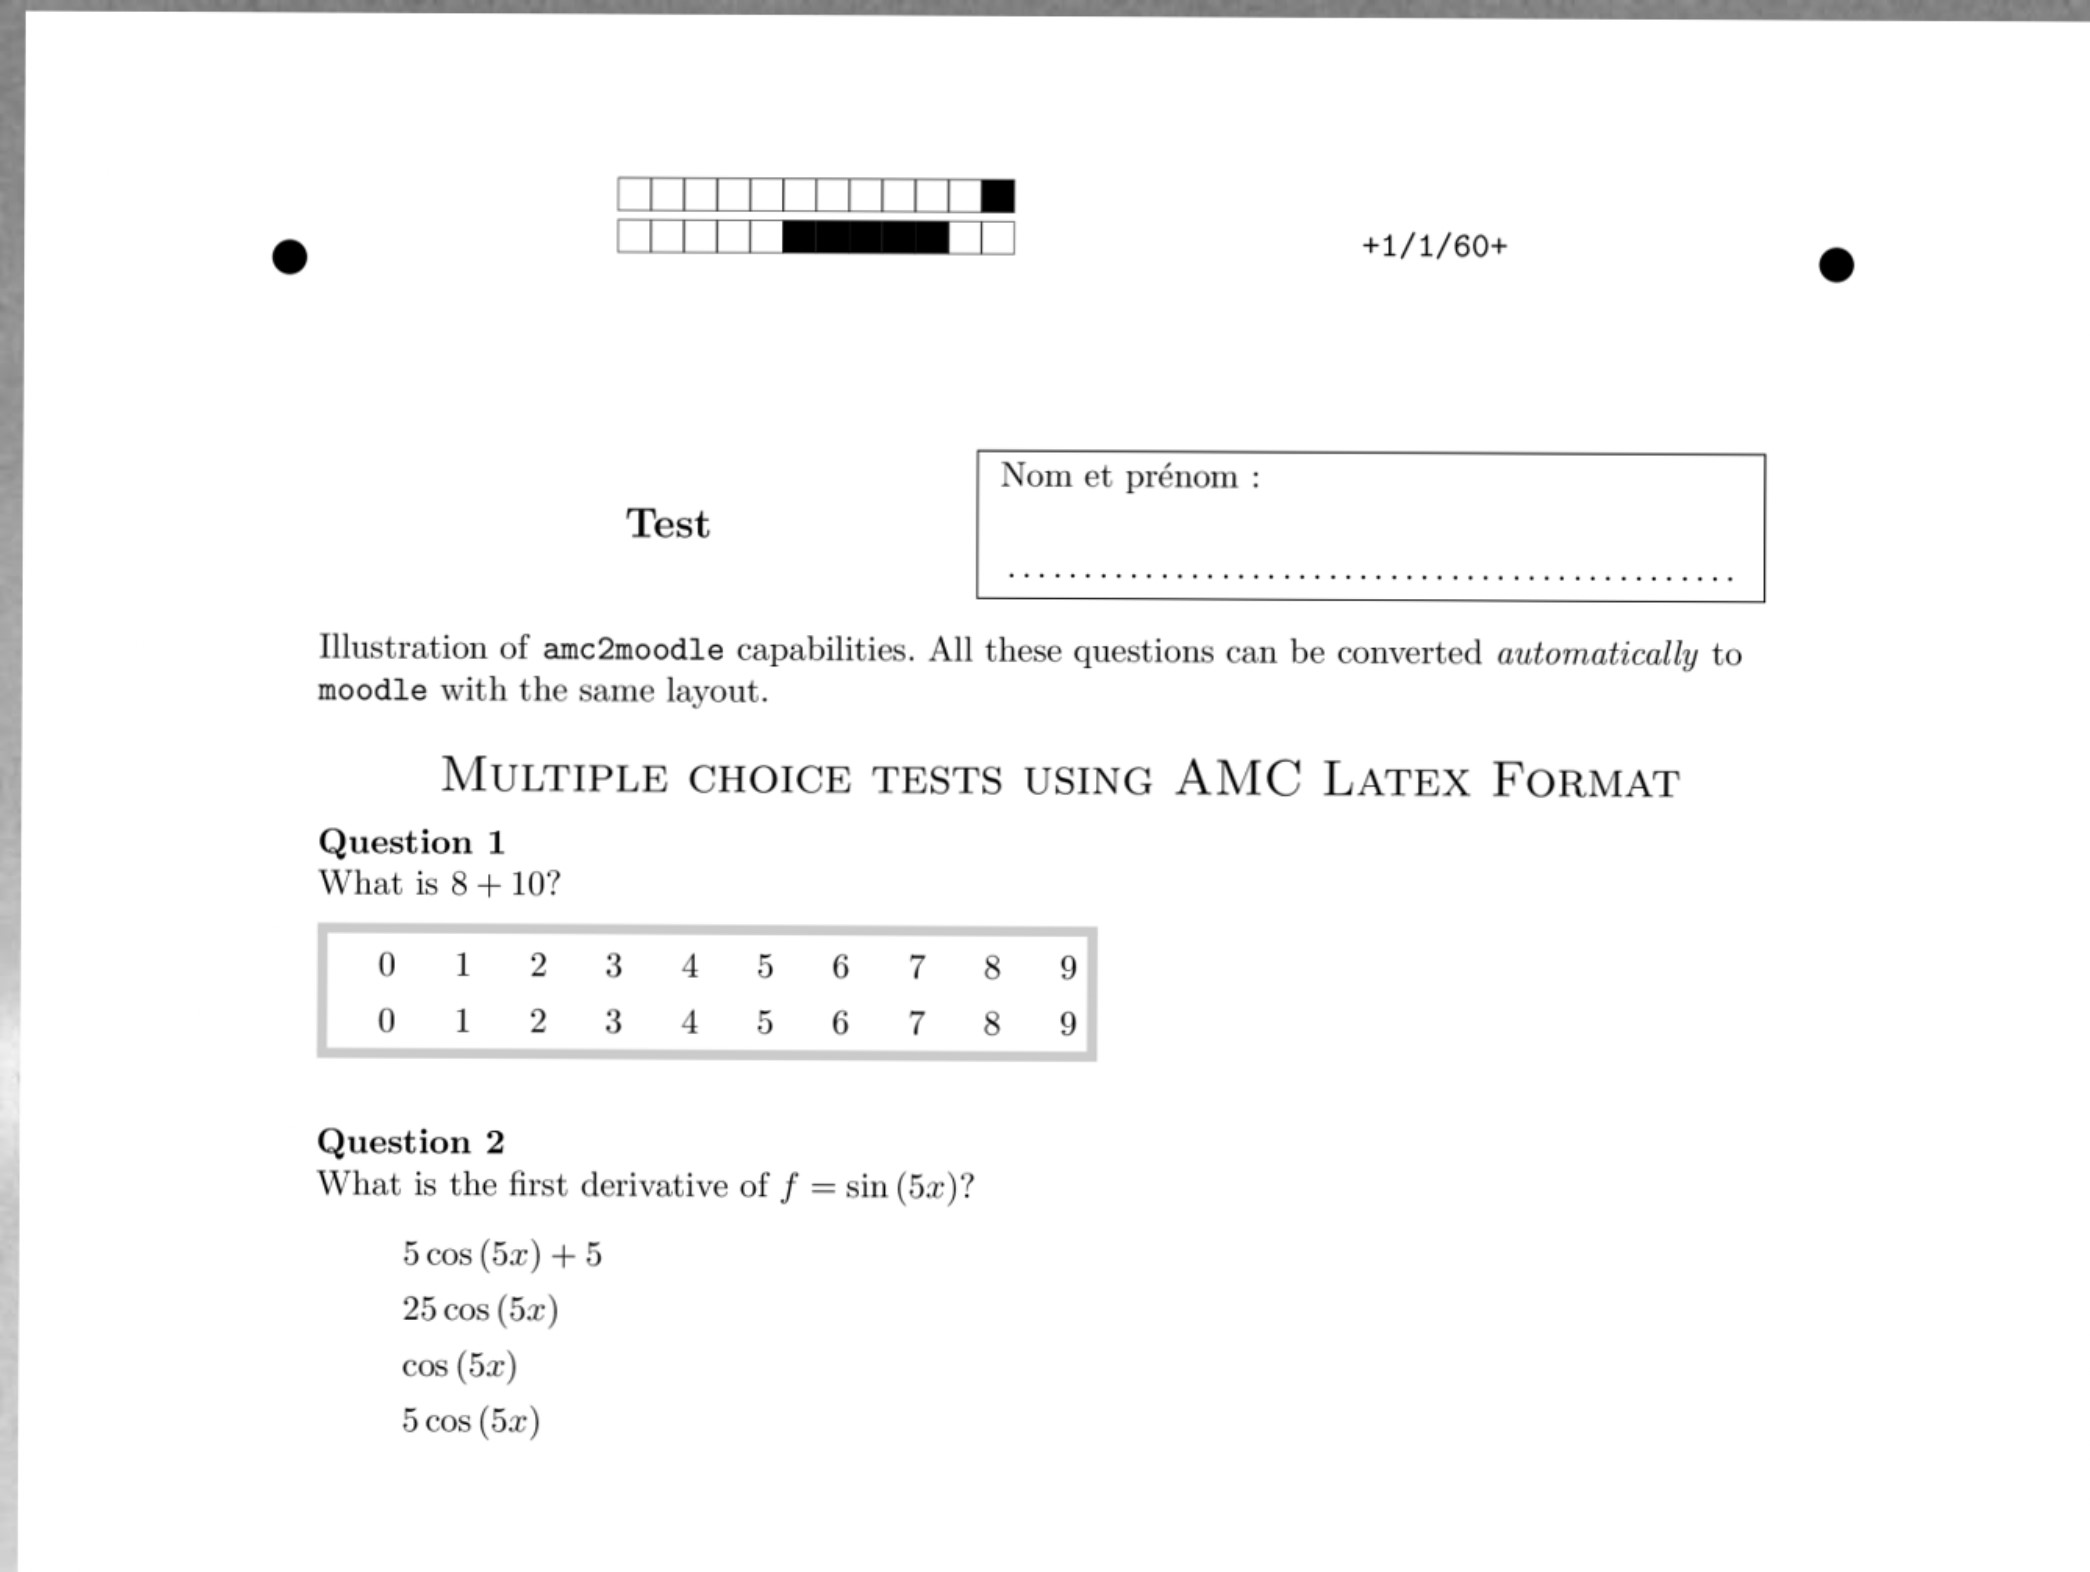
\includegraphics[width=0.9\textwidth]{figures/scan11111_cut.jpg}
    \caption{Escaneo generado sin casillas}
    \label{fig:fscan_bad}
\end{figure}
            \item El problema parece ser por los forms, asi que primero imprimo el statement rellenado a otro fichero pdf y luego vuelvo a generar el escaneo (\ref{fig:fscan_good})
\begin{figure}
    \centering
    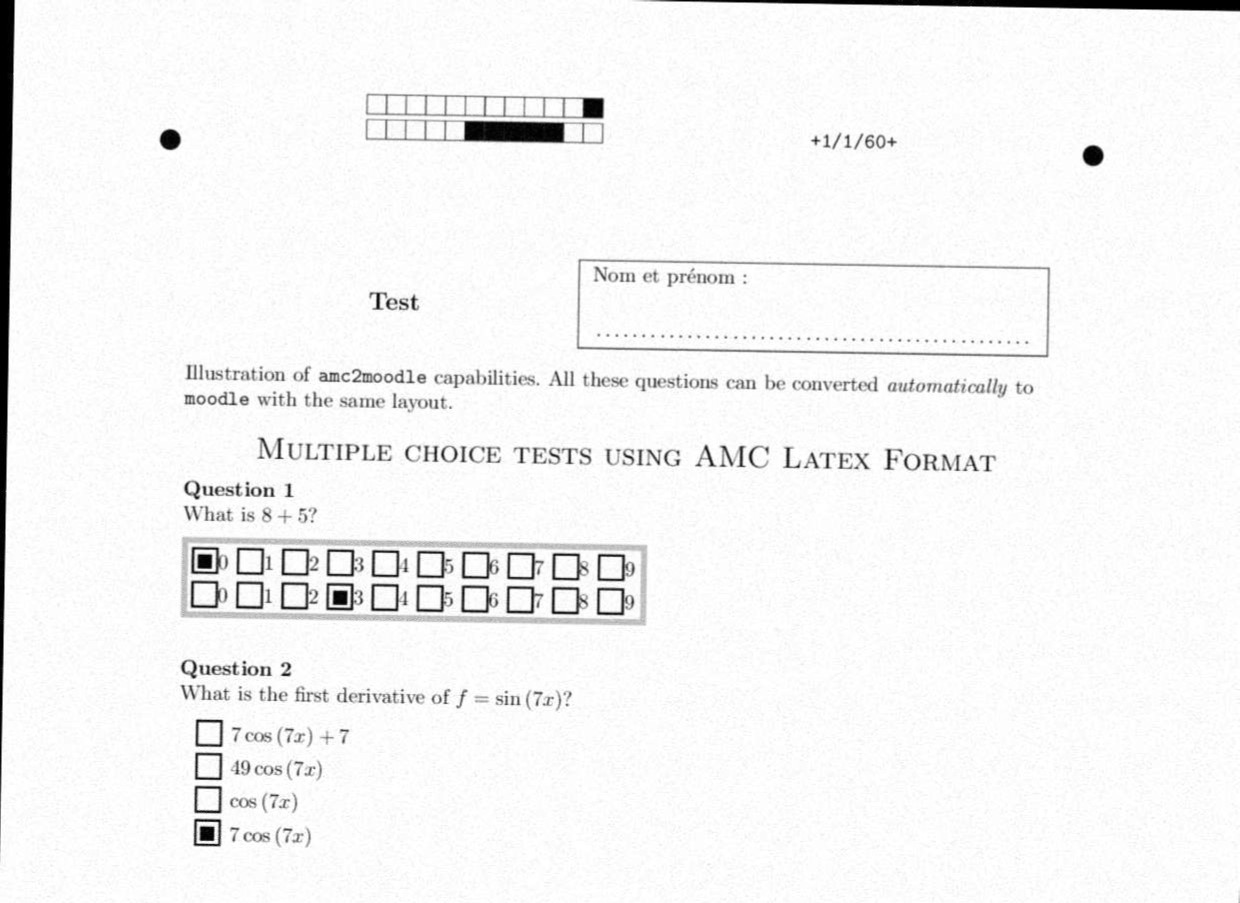
\includegraphics[width=0.9\textwidth]{figures/s_11111_cut.jpg}
    \caption{Escaneo generado correctamente}
    \label{fig:fscan_good}
\end{figure}
            \item Ajusto los parámetros de i2pdf para que los escaneados tengan calidades distintas
        \end{itemize}
        \item 
    \end{itemize}
\end{itemize}

Semana 13-20 DIC, TODO:

\begin{itemize}
    \item Leer y escribir JSONs desde python
    \item Exportar paginas pdf a png
    \item 
\end{itemize}
